
\section{Graph Representation}
\begin{wrapfigure}{r}{0.5\textwidth}
	\begin{center}
		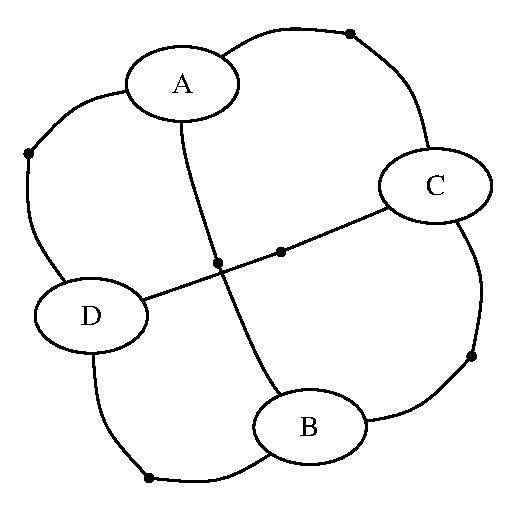
\includegraphics[width=0.5\textwidth]{FullGraph.eps}
	\end{center}
\end{wrapfigure}

A fully connected undirected graph where every node is connected to every node is represented correctly by assigning the numbers that come in the second position of the odometer to values equal to the first position plus one. \\

When the restriction is removed the representation changes to be equivalent to representing a fully connected digraph where every there is a directional edge from every node to every node. 
\begin{lstlisting}
def OdometerAsFullUndirectedGraph(hypergraph,odometer):
if len(odometer) == 2:
if odometer[1] + 1 < len(hypergraph):
odometer[1] += 1
return True
else:
if odometer[0] + 2 < len(hypergraph):
odometer[0] += 1
odometer[1] = odometer[0] +1
return True
return False
\end{lstlisting}

\begin{center}
	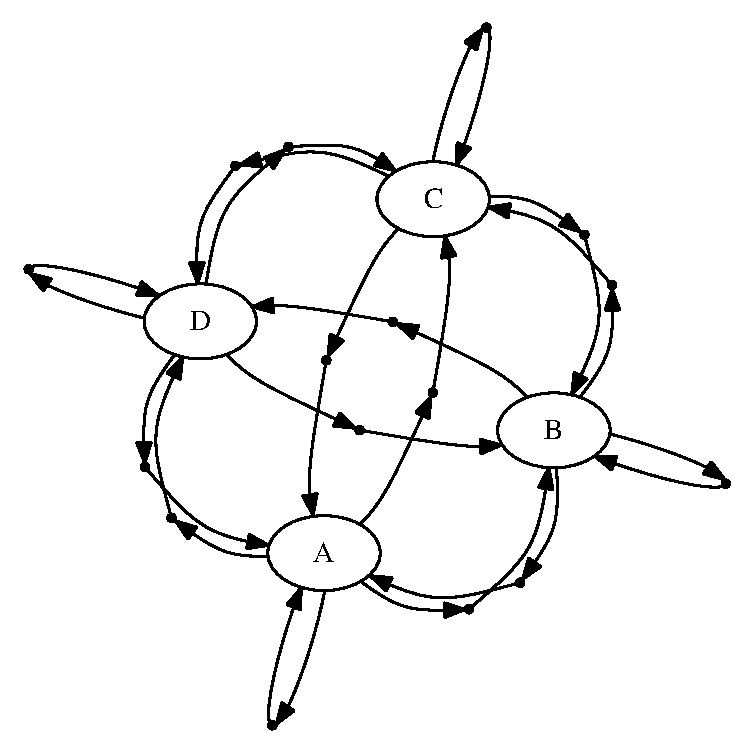
\includegraphics[width=0.5\textwidth]{FullDirectedGraph.eps}
\end{center}

\begin{lstlisting}
def OdometerAsFullDirectedGraph(hypergraph,odometer):
if len(odometer) == 2:
if odometer[1] + 1 < len(hypergraph):
odometer[1] += 1
return True
else:
if odometer[0] + 1 < len(hypergraph):
odometer[0] += 1
odometer[1] = 0
return True
return False
\end{lstlisting}

Notice that the restriction lifting now gives allows the edge $\{A \rightarrow A\}$ which has mathematical relevance but may make no sense in the context of the graph being interpreted. Thus selecting the correct mathematical representation as an expressive function that restricts the domain properly is critical in ensuring the enumeration represents the correct model. The function which advances odometers both defines what the next discrete point in the space will be and also sets the bounds of the mathematical space.

\newpage


\section{Forest of Trees}
\section{Uniform selection from multiple variables}
Sampling $N$ items from a set which is larger than is feasible to compute is a complex problem as the quality of sample points is a significant factor in the quality of the final data set. Each variable has a domain of values that can be mapped to a hypergraph. A vector of numbers is computed that contains the size of the domain of each variable. Each index in the odometer represents the index in the vector of hypergraphs. Each value in the odometer represents the node to select from the hypergraph. Thus there is only one value selected for each variable for a given odometer. \\

Odometers can map a space of size ${\Pi_{i=1}^{V} D_i}$ unto a single dimensional number line-path. This path can then be sliced into the number of samples. The odometer is advanced by the distance between sample points on the number line. This transformation is linear-polynomial to take $N$ samples from a mapping whose size exceeds the size of the universe. 
\newpage

\begin{lstlisting}
def getNextSampleOdometer(odometer,odometer_state,domain_sizes,step_size):
    control = 0
    domain_size = mul_list(domain_sizes)
    step_size = step_size % domain_size

    while control < len(odometer):
        size = domain_sizes[control]
        step = step_size % size
        step_size = step_size // size
        cur_num = odometer[control]
        dir_num = odometer_state[control]

        if step_size %2 == 1:
            cur_num = (size - 1) - cur_num
            if dir_num == 1:
                dir_num = -1
            else:
                dir_num = 1

        cur_num = cur_num + dir_num * step

        if cur_num < 0:
            cur_num +=1
            dir_num = 1
            cur_num = (size-1) - cur_num
            step_size +=1
        if cur_num >= size:
            dir_num =-1
            cur_num = (size-1) - (cur_num - size)
            step_size +=1

        odometer[control] = cur_num
        odometer_state[control] = dir_num

        if step_size == 0:
            return
        control+=1
    return
\end{lstlisting}
\newpage
